

\chapter{DCM for fNIRS \label{Chap:data:fnirs}}

Functional near-infrared spectroscopy (fNIRS) is a noninvasive method for monitoring hemodynamic changes in the brain via measurements of optical absorption changes \cite{jobsis1977noninvasive}. As neuronal process requires extra delivery of oxygen, this hemodynamic change provides a marker of underlying neuronal activity. \\

As compared to fMRI, fNIRS provides a more direct measure of changes in oxygenated, deoxygenated, and total hemoglobin (HbO, HbR, and HbT) with high temporal resolution. However, due to complex relationships between neurodynamic and hemodynamic processes, functional connectivity often differs with the type of hemodynamic changes (e.g., HbO and HbR), while underlying interactions between neuronal populations do not vary. This highlights the importance of estimating causal influences among neuronal populations, referring to a biophysical model of how neuronal activity is transformed into fNIRS measurements. \\

DCM for fNIRS allows for making inference about changes in directed connectivity at the neuronal level from the measurement of optical density changes \cite{tak2015dynamic}. DCM is a framework for fitting differential equation models of neuronal activity to brain imaging data using Bayesian inference \cite{Friston2003a, Friston2007a, families}. Because the Bayesian estimation is the same as the one used for DCMs for other imaging modalities \cite{Friston2007a, families}, the main differences are a generative model describing how observed fNIRS data are caused by the interactions among hidden neuronal states. \\

In particular, the neurodynamic and hemodynamic models used for DCM-fMRI analysis \cite{Friston2003a} are extended to addtionally include the following components:
\begin{itemize} 
\item In the hemodynamic model, \emph{the rate of HbT changes} $\dot{p}_j$, \cite{cui10}, is modeled as:
\begin{eqnarray} 
\tau_j \dot{p}_j  =  \left(f_{j,in} - f_{j,out}\right)\frac{p_j}{v_j},
\end{eqnarray}
where $j$ denotes cortical source region, $f_{j,in}$ is inflow, $f_{j,out}$ is outflow, $v_j$ is blood volume, and $\tau_j$ is the transit time. 

\item \emph{An optics model} relates the hemodynamic sources to measurements of optical density changes \cite{delpy1988estimation, arridge1999optical}. Optical density changes at channel $i$ and wavelength $\lambda$, $y_i(\lambda)$, are described as a linear combination of light absorption changes due to hemoglobin oxygenation: 
\begin{eqnarray}\label{eq:optics} 
y_i (\lambda) = \frac{1}{\omega_{i,H}} \sum_{i=1}^{N} S_{i,j}(\lambda)\epsilon_H(\lambda) \Delta H_{j,c} +  \frac{1}{\omega_{i,Q}} \sum_{i=1}^{N} S_{i,j}(\lambda)\epsilon_Q(\lambda) \Delta Q_{j,c}
\end{eqnarray} 
where $\Delta H_{j,c}$ and $\Delta Q_{j,c}$ are the HbO and HbR changes in the cortical source region $j$; $S(\lambda)$ is the sensitivity matrix at wavelength $\lambda$; $\epsilon_H$ and $\epsilon_Q$ are the extinction coefficients for HbO and HbR; $\omega = \frac{\mathrm{cortical}}{\mathrm{cortical} + \mathrm{pial}}$ is a factor for correcting the effect of pial vein oxygenation changes on fNIRS measurements  \cite{gagnon2012quantification}. 

\item \emph{Spatially extended hemodynamic sources}. In the optics model (Eq.~\ref{eq:optics}), each hemodynamic signal is modelled as a point source which produces a hemodynamic response at a single specified anatomical location. However, the hemodynamic response can be spatially extended. Hemodynamic activity at a source location is then specified by convolving the temporal response with a Gaussian spatial kernel.

\end{itemize} 

\section{Example: Motor Execution and Imagery Data} 
This section presents an illustrative DCM analysis using fNIRS data acquired during the motor execution and motor imagery tasks. This data was collected by Agnieszka Kempny and Alex Leff in Royal Hospital for Neuro-disability, and is available from the SPM website\footnote{\url{http://www.fil.ion.ucl.ac.uk/spm/data/fnirs/}}.

\subsection*{Experimental protocol}
\begin{itemize}
\item In the first session, the subject was instructed to squeeze and release a ball with her right hand during task blocks. In the second session, the subjected was instructed to perform kinesthetic imagery of the same hand movement, but without moving the hand. 
\item For both sessions, there were 5 second blocks of tasks where the cue was presented with an auditory beep, interspersed with 25 second rest blocks. 
\item A previous study found consistent activation in the supplementary motor area (SMA) and premotor cortex during motor execution and imagery, and reduced activation in primary motor cortex (M1) during motor imagery \cite{hanakawa2003functional}. Moreover, a recent study has revealed, using DCM for fMRI \cite{kasess2008suppressive}, that coupling between SMA and M1 may serve to attenuate the activation of M1 during motor imagery. 
\item In this manual, using DCM-fNIRS, we investigate (i) how the motor imagery condition affects the directed connections between SMA and M1, and (ii) how these interactions are associated with the regional activity in M1 and SMA during motor execution and imagery.
\end{itemize}

\section{SPM Analysis}
Prior to DCM analysis, brain regions whose dynamics are driven by experimental conditions are identified using a standard SPM analysis\footnote{The first-level fNIRS analysis. including preprocessing, artefact removal, general linear modelling, spatial registration were all implemented using the SPM for fNIRS toolbox. This is available from \url{https://www.nitrc.org/projects/spm_fnirs/.} See the toolbox manual for more details.}. Using motor execution and imagery data, we can find that SMA is significantly activated during both motor execution and motor imagery, whereas M1 is only activated during motor execution. The most significantly activated voxels within SMA and M1 are then selected as the source positions for DCM analysis: The MNI coordinates are: SMA, $[51, 4, 55]$; and M1, $[44, 16, 65]$.

\section{Specifying and Estimating the DCM}
Now we will generate a connectivity model of how observed fNIRS data are caused by interactions among hidden neuronal states. Specifically, we will determine (i) which regions receive driving input, (ii) which regions are connected in the absence of experimental input, and (iii) which connections are modulated by input. In this example, we will generate the best model (selected using Bayesian model comparison) in which task input could affect regional activity in both M1 and SMA, and motor imagery modulates both extrinsic and intrinsic connections. 

\begin{enumerate} 
\item After starting SPM in the EEG modality, add the DCM for fNIRS toolbox to the MATLAB path:\\
>> \texttt{addpath(fullfile(spm('Dir'),'toolbox','dcm\_fnirs'))}
\item Type \texttt{spm\_dcm\_fnirs\_specify} at the MATLAB command window. \\
>> \texttt{spm\_dcm\_fnirs\_specify};
\item Select the \texttt{SPM.mat} files that were created when specifying the GLM. \\
eg, \texttt{fnirs\_data/ME/SPM.mat}, and \texttt{fnirs\_data/MI/SPM.mat}.
\item Highlight `name for DCM\textunderscore???.mat' and enter a DCM file name you want to create eg, \texttt{fully\_connected}.
\item Select a directory, eg. \texttt{fnirs\_data}, in which to place the results of your DCM analysis.
\item \textbf{Preprocess time series of optical density changes}
\begin{enumerate} 
\item Highlight `temporal filtering? [Butterworth IIR/No]'. \\Select the Butterworth IIR button to reduce very low-frequency confounds, and physiological noise eg, respiration and cardiac pulsation.
\begin{itemize}
\item Highlight `stopband frequencies Hz [start end]', and then accept the default value `[0 0.008; 0.12 0.35; 0.7 1.5]'.
\end{itemize}
\item Highlight `average time series over trials?'. \\Select `yes' to average the optical density signal across trials, and then specify averaging window length [secs] for each experimental condition. 
\begin{itemize} 
\item Highlight `for motor execution:' and change the default values 30.2683 to 30. 
\item Highlight `for motor imagery:' and change the default values 30.6624 to 30. 
\end{itemize}
\end{enumerate}
\item \textbf{Specify confounding effects}
\begin{enumerate}
\item Highlight `regressors? [DCT/User/None]'. \\ Select `DCT' to model confounding effects (eg, Mayer waves) using a discrete cosine transform set. 
\begin{itemize}
\item Highlight `periods [sec]', and then accept the default value `[8 12]'. 
\end{itemize}
\item Highlight `correction of pial vein contamination? [yes/no'].\\ Select `yes' to correct pial vein contamination of fNIRS measurements.
\end{enumerate}

\item \textbf{Specify fNIRS channels to be used in DCM}.
\begin{enumerate}
\item Highlight `use all sensor measurements? [yes/no]'.\\Select `no' to specify sensor (channel) measurements to be used in DCM analysis. 
\begin{itemize}
\item Highlight `sensors of interest', and enter eg, [1 2 3 4 9 10 11 12] \\Only fNIRS data from the left hemisphere is used in this study. You can refer to sensor positions shown in `Figure 1: Optode and Channel Positions'.
\end{itemize}
\end{enumerate}
\item \textbf{Specify hemo/neurodynamic source positions}.
\begin{enumerate}
\item Enter total number of sources to be estimated using DCM eg, 2. 
\begin{itemize}
\item Enter a name of source 1 eg, M1
\item Enter MNI coordinates of source 2 eg, [$-$44 $-$16 65]
\item Enter a name of source 2 eg, SMA
\item Enter MNI coordinates of source 1 eg, [$-$51 $-$4 55]
\end{itemize}
\item Highlight `type of hemodynamic source [Point/Distributed]' \\Select 'Distributed' to use spatially extended hemodynamic source rather than point source. 
\begin{itemize}
\item Highlight `radius of distributed source [mm]', and accept the default value `4'. 
\end{itemize}
\end{enumerate}
\item Select a file containing Green's function of the photon fluence precomputed using the mesh-based Monte Carlo simulation software (MMC, \cite{fang2010mesh}\footnote{We provide a code for estimating Green's function based on the MMC software. The code currently only runs on Mac OS.} eg, \texttt{fnirs\_data/greens/est\_G.mat}.
\item \textbf{Input Specification}
\\Specify experimental input that modulates regional activity and connectivity. 
\begin{enumerate}
\item Highlight `number of conditions/trials', and then enter `2'. 
\item Highlight `name for condition/trial1?', and enter `motor task'. \\'motor task' encodes the occurrence of motor execution and motor imagery tasks. 
\begin{itemize}
\item Highlight `onsets - motor task [sec]', and enter `[0 30]'. 
\item Highlight `duration[s] [sec]', and enter `5'. 
\end{itemize}
\item Highlight `name for condition/trial2?', and enter `motor imagery'. 
\begin{itemize}
\item Highlight `onsets - motor task [sec]', and enter `30'. 
\item Highlight `duration[s] [sec]', and enter `Inf'. 
\end{itemize}
\end{enumerate}
\item \textbf{Specify endogenous (fixed) connections}
\begin{itemize}
\item Define connections in the absence of input: M1 to SMA, SMA to M1. \\Your connectivity matrix should look like the one in Fig.~\ref{fig:gui_con}.
\end{itemize}
\item \textbf{Specify regions receiving driving input}
\begin{itemize}
\item Highlight `Effects of motor tasks on regions and connections', and specify motor tasks as a driving input into M1 and SMA. See Fig.~\ref{fig:gui_con}.
\end{itemize}
\item \textbf{Specify connections modulated by input}
\begin{itemize}
\item Highlight `Effects of motor imagery on regions and connections. \\Specify motor imagery to modulate intrinsic connections on M1 and SMA; extrinsic connections from M1 to SMA, and from SMA to M1. See Fig.~\ref{fig:gui_con}. 
\end{itemize}
A polite ``Thank You'' completes the model specification process. A file called \texttt{DCM\_fully\_connected.mat} will have been generated. 
\item You can now estimate the model parameters by typing \\
>> \texttt{spm\_dcm\_fnirs\_estimate};
\item Select the DCM.mat file created in the last step eg, \texttt{fnirs\_data/DCM\_fully\_connected.mat}. After convergence of estimation of DCM parameters, results will appear in a window, as shown in Fig.~\ref{fig:fit}. 

\begin{itemize}
\item Also, you can display DCM analysis results, including connectivity parameters, estimated neural responses, and DCM fit, by typing \\ 
>> \texttt{spm\_dcm\_fnirs\_viewer\_result};
\item Select the DCM.mat file eg, \texttt{fnirs\_data/}, and then results will appear in a window, as shown in Figs.~\ref{fig:est_conn} and \ref{fig:est_neural}. 
\end{itemize}
\end{enumerate}

\newpage
\begin{figure}
\begin{center}
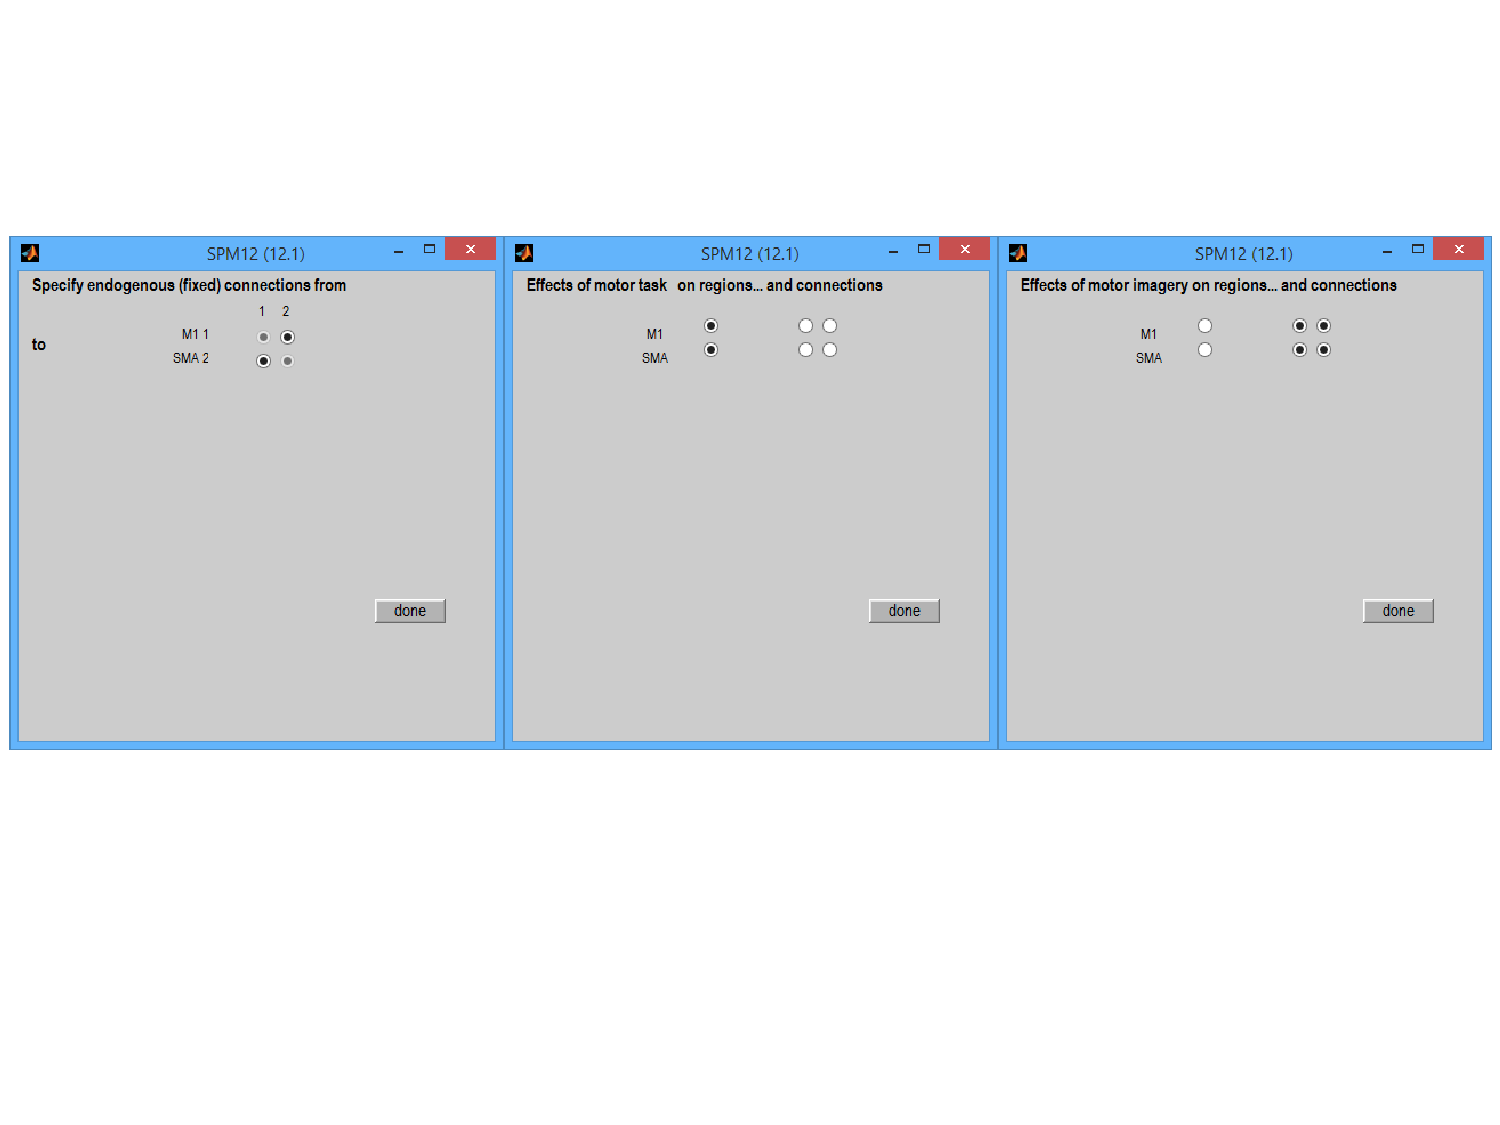
\epsfig{file=dcm_fnirs/figs/gui_con,width=14cm}
\caption{Specification of model depicted in Fig.7 \cite{tak2015dynamic}. In this model, motor task input affects regional activity in both M1 and SMA, and motor imagery modulates both extrinsic and intrinsic connections. Left: Endogenous (fixed) connections. Middle: Regions receiving driving input (eg, motor tasks encoding the occurrence of motor execution and motor imagery tasks). Right: Connections modulated input (eg, motor imagery task).\label{fig:gui_con}}
\end{center}
\end{figure}


\newpage
\begin{figure}
\begin{center}
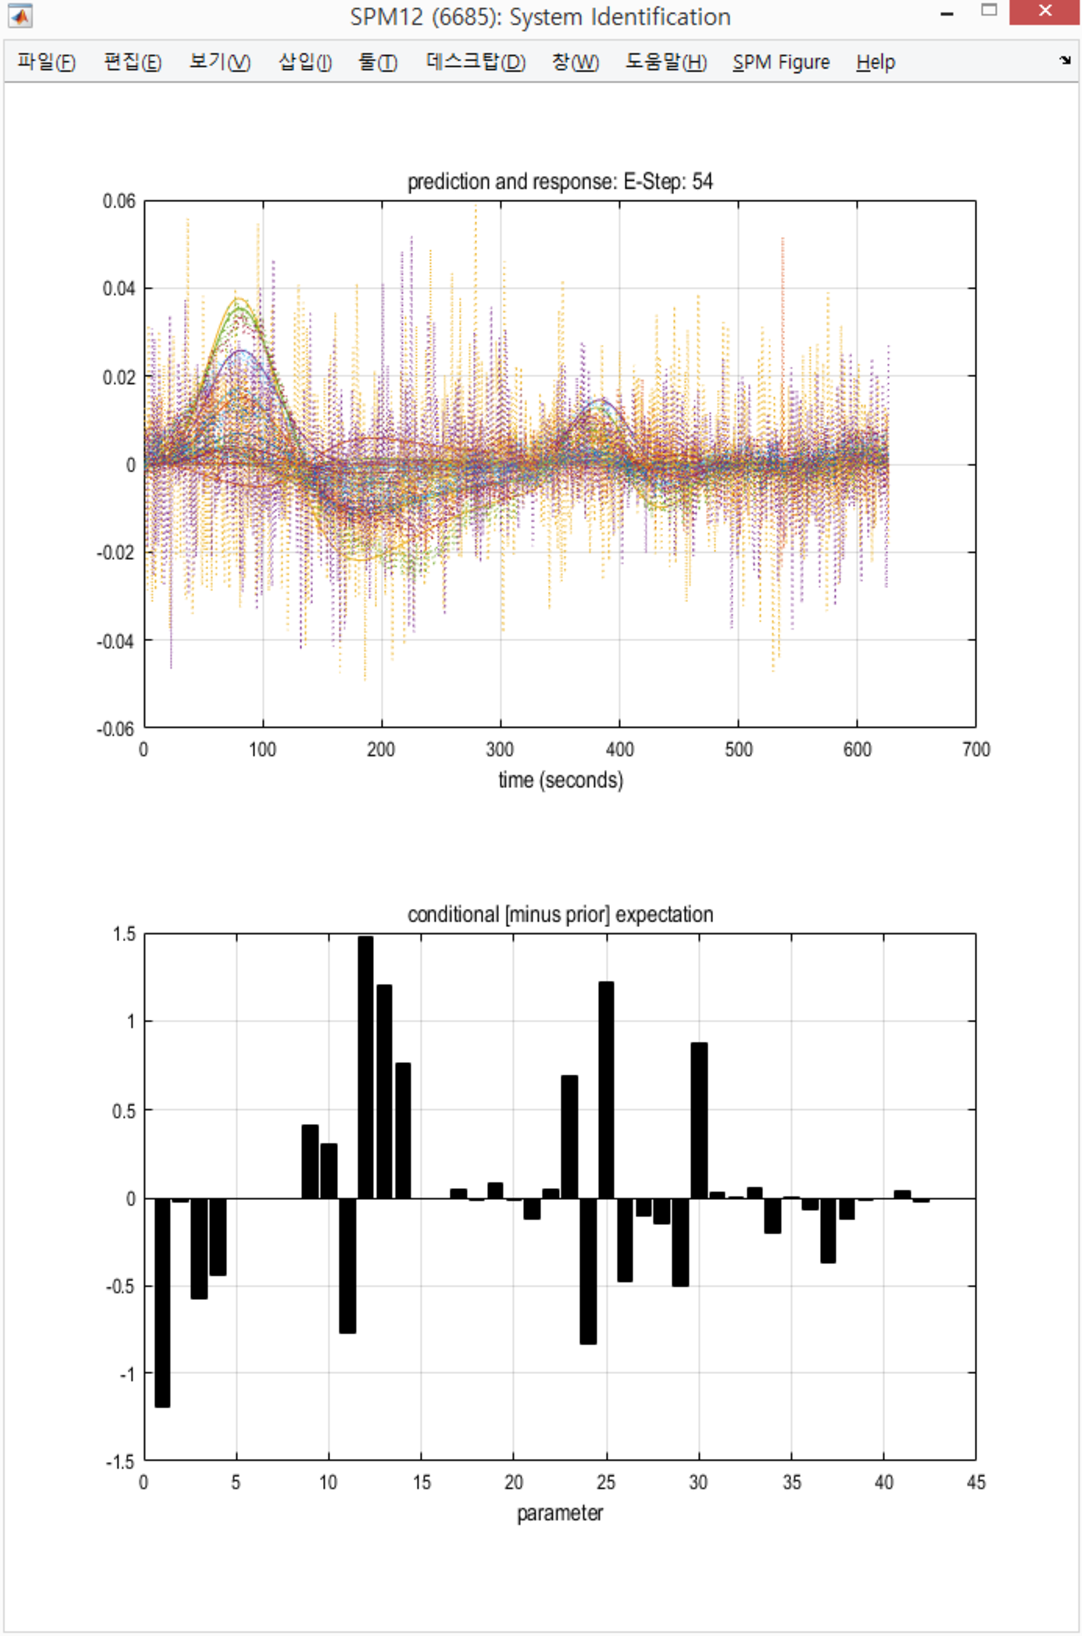
\epsfig{file=dcm_fnirs/figs/dcm_fit,width=13cm}
\caption{Results of estimation of DCM parameters. Top: Predicted and observed response, after convergence. Bottom: Conditional expectation of the parameters.\label{fig:fit}}
\end{center}
\end{figure}


\newpage
\begin{figure}
\begin{center}
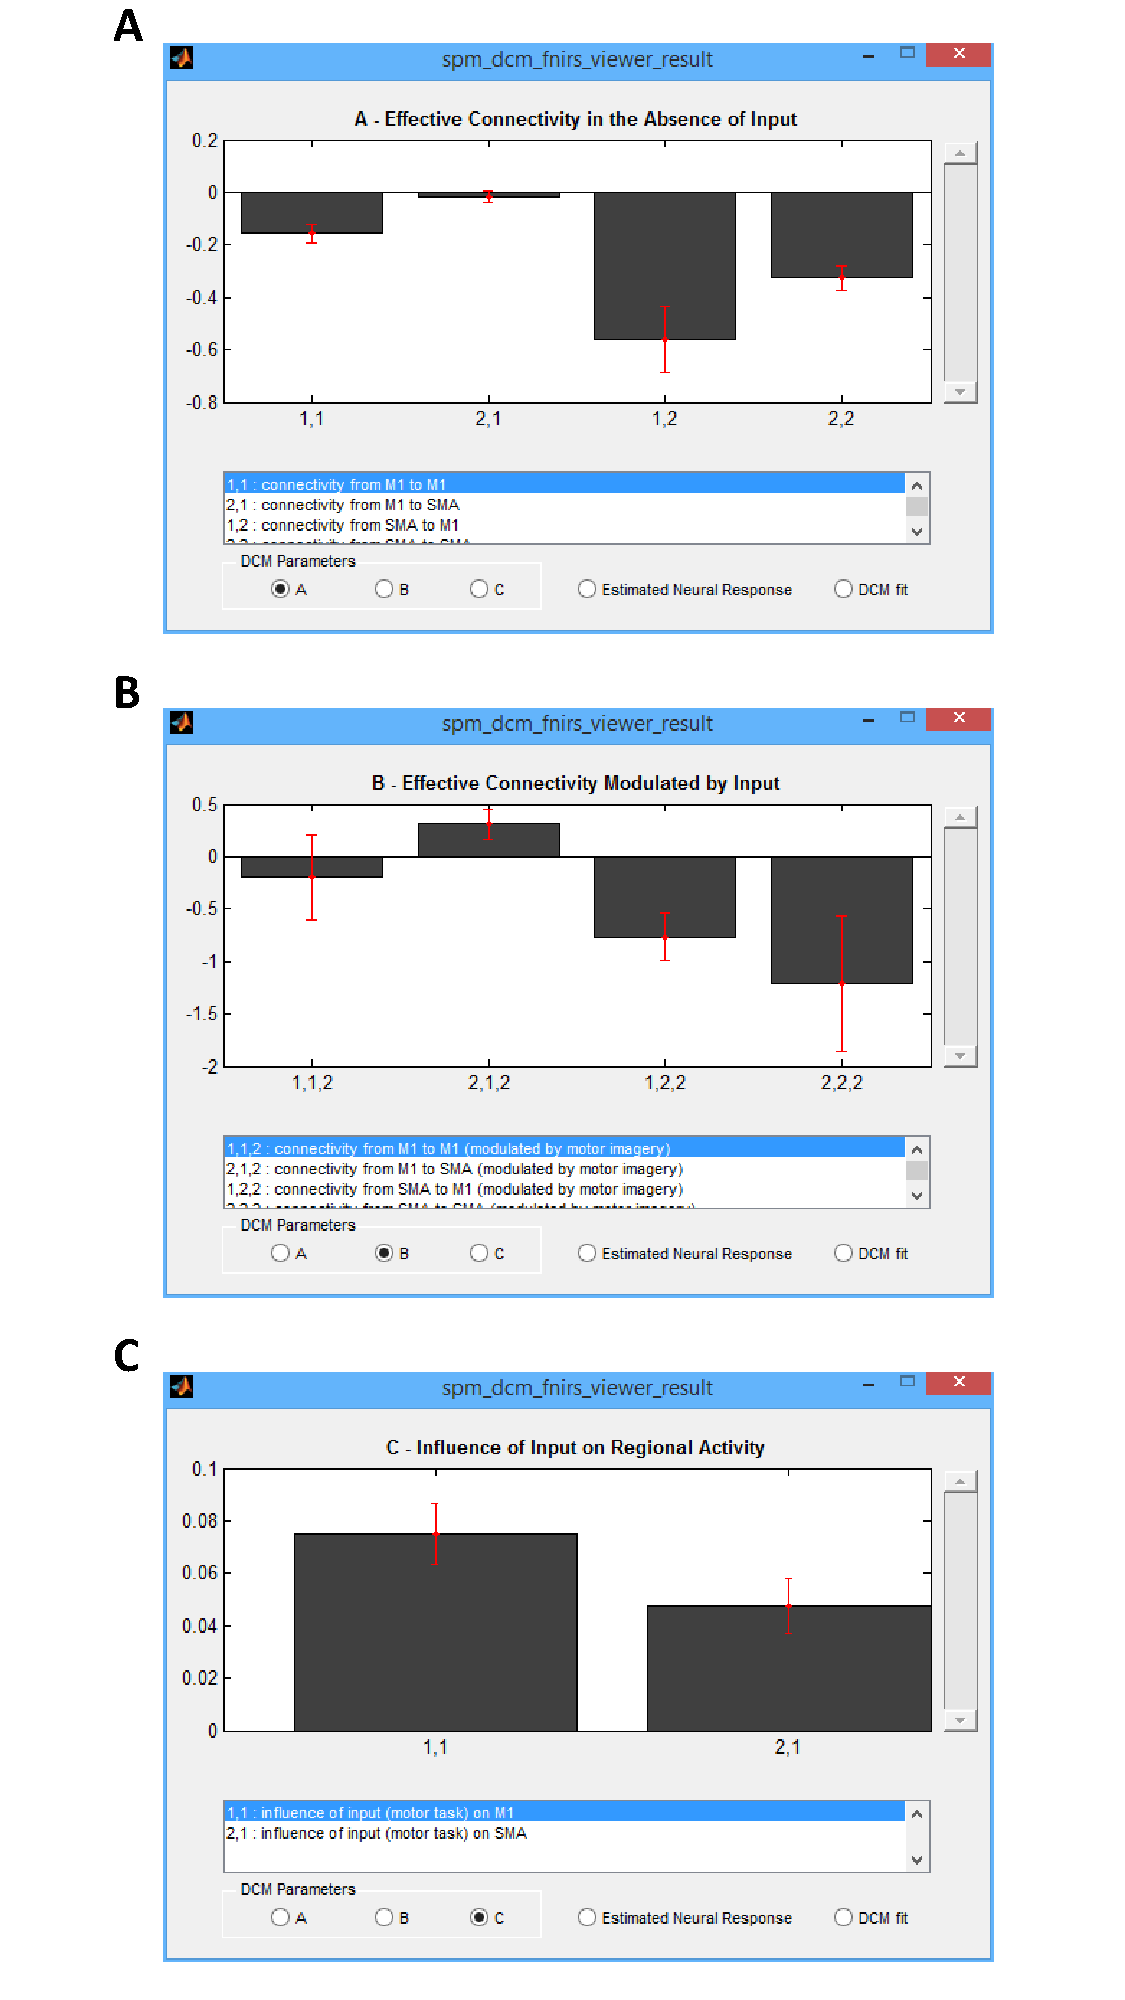
\epsfig{file=dcm_fnirs/figs/est_conn,width=13cm}
\caption{Estimated parameters of effective connectivity. These results indicate that while all motor stimuli positively affect theregional activity in primarymotor cortex (M1), motor imagery negativelymodulates connection fromsupplementarymotor area (SMA) to M1, resulting in the suppressive influence of SMA on M1. See \cite{tak2015dynamic} for more details. \label{fig:est_conn}}
\end{center}
\end{figure}

\newpage
\begin{figure}
\begin{center}
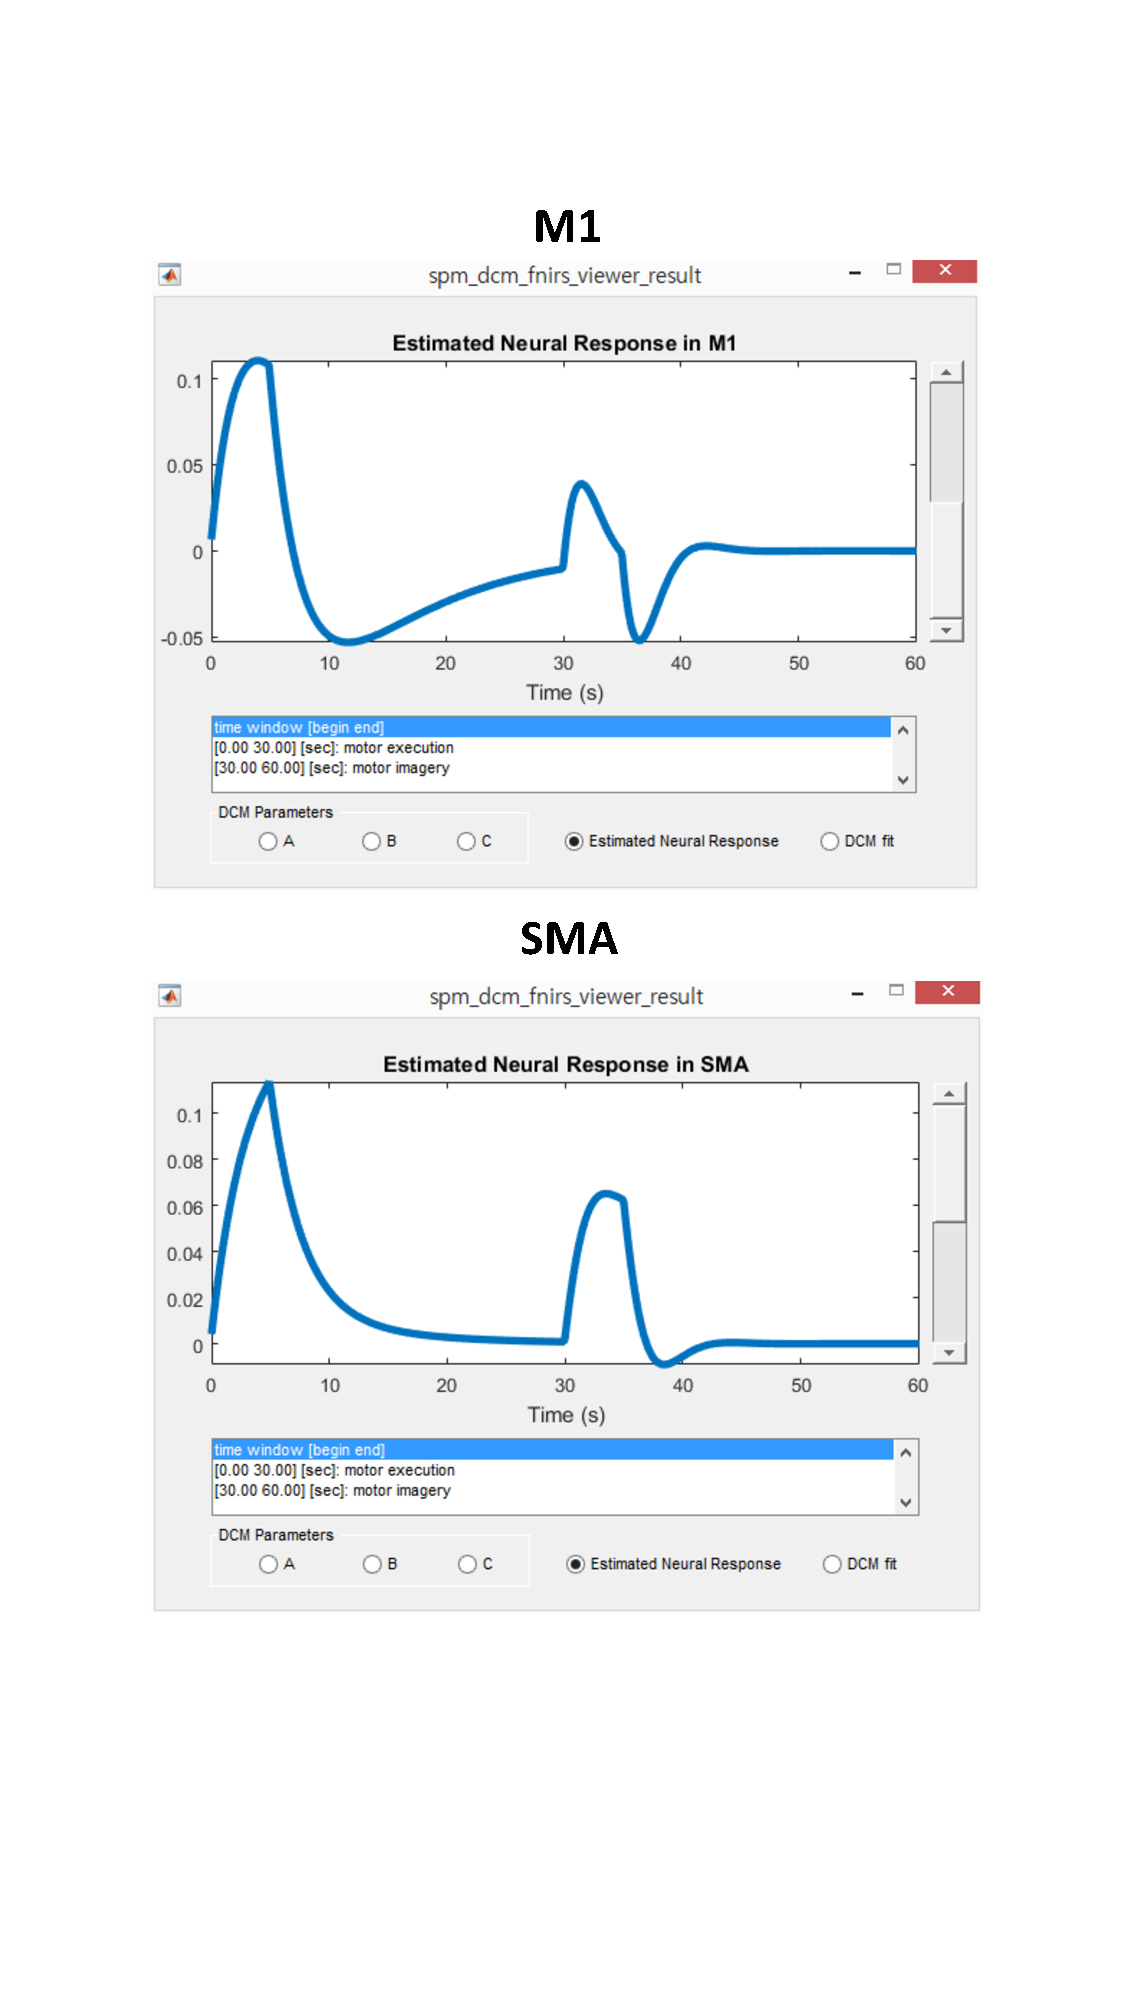
\epsfig{file=dcm_fnirs/figs/est_neural,width=13cm}
\caption{Estimated neural responses. Duringmotor imagery, neural activity in primary motor cortex (M1) is significantly reduced, while neural activity in supplementary motor area (SMA) is relatively consistent, compared with activity during motor execution.\label{fig:est_neural}}
\end{center}
\end{figure}


\clearpage

\begin{thebibliography}{10}

\bibitem{jobsis1977noninvasive}
F.~F. Jobsis.
\newblock Noninvasive, infrared monitoring of cerebral and myocardial oxygen
  sufficiency and circulatory parameters.
\newblock {\em Science}, 198(4323):1264--1267, 1977.

\bibitem{tak2015dynamic}
S.~Tak, A.~Kempny, K.~Friston, A.~Leff, and W.~Penny.
\newblock Dynamic causal modelling for functional near-infrared spectroscopy.
\newblock {\em Neuroimage}, 111:338--349, 2015.

\bibitem{Friston2003a}
K.~J. Friston, L.~M. Harrison, and W.~D. Penny.
\newblock Dynamic causal modelling.
\newblock {\em Neuroimage}, 19(4):1273--1302, 2003.

\bibitem{Friston2007a}
K.~J. Friston, J.~Mattout, N.~Trujillo-Barreto, J.~Ashburner, and W.~D. Penny.
\newblock Variational free energy and the {Laplace} approximation.
\newblock {\em Neuroimage}, 34(1):220--234, 2007.

\bibitem{families}
W.~Penny, K.~E. Stephan, J.~Daunizeau, M.~J. Rosa, K.~J. Friston, T.~M.
  Schofield, and A.~P. Leff.
\newblock Comparing families of dynamic causal models.
\newblock {\em PLoS Comput. Biol.}, 6(3):e1000709, 2010.

\bibitem{cui10}
X.~Cui, S.~Bray, and A.~L. Reiss.
\newblock {Functional near infrared spectroscopy (NIRS) signal improvement
  based on negative correlation between oxygenated and deoxygenated hemoglobin
  dynamics}.
\newblock {\em {NeuroImage}}, 49:3039--3046, 2010.

\bibitem{delpy1988estimation}
D.~T. Delpy, M.~Cope, P.~Van~der Zee, S.~Arridge, S.~Wray, and J.~Wyatt.
\newblock Estimation of optical pathlength through tissue from direct time of
  flight measurement.
\newblock {\em Phys. Med. Biol.}, 33(12):1433--1442, 1988.

\bibitem{arridge1999optical}
S.~R. Arridge.
\newblock {Optical tomography in medical imaging}.
\newblock {\em Inverse Probl.}, 15:R41--R93, 1999.

\bibitem{gagnon2012quantification}
L.~Gagnon, M.~A. Y{\"u}cel, M.~Dehaes, R.~J. Cooper, K.~L. Perdue, J.~Selb,
  T.~J. Huppert, R.~D. Hoge, and D.~A. Boas.
\newblock {Quantification of the cortical contribution to the NIRS signal over
  the motor cortex using concurrent NIRS-fMRI measurements}.
\newblock {\em NeuroImage}, 59(4):3933--3940, 2012.

\bibitem{hanakawa2003functional}
T.~Hanakawa, I.~Immisch, K.~Toma, M.~A. Dimyan, P.~Van~Gelderen, and
  M.~Hallett.
\newblock {Functional properties of brain areas associated with motor execution
  and imagery}.
\newblock {\em J. Neurophysiol.}, 89:989--1002, 2003.

\bibitem{kasess2008suppressive}
C.~H. Kasess, C.~Windischberger, R.~Cunnington, R.~Lanzenberger, L.~Pezawas,
  and E.~Moser.
\newblock {The suppressive influence of SMA on M1 in motor imagery revealed by
  fMRI and dynamic causal modeling}.
\newblock {\em Neuroimage}, 40:828--837, 2008.

\bibitem{fang2010mesh}
Q.~Fang.
\newblock {Mesh-based Monte Carlo method using fast ray-tracing in Pl{\"u}cker
  coordinates}.
\newblock {\em Biomed. Opt. Express}, 1:165--175, 2010.

\end{thebibliography}

%----------------------------------------------------------------------------------------
